
\chapter{Ergebnisse}

\section{Bildqualität}
Hardwarebedingt ist es uns nicht m\"oglich aussagekr\"aftige Bilder 
gegen\"uberzustellen. Durch Verringer der Kamerafrequenz wird die Bildqualit\"at bereits erheblich reduziert. 

Sowohl bei 2D wie auch bei 3D Komprimierung sind die Artefakte sichtbar,
die sich auf dem Bild befindende Objekte sind aber gut erkennbar:

\begin{figure}[htpb]
\begin{center}
\subfigure[RAW]{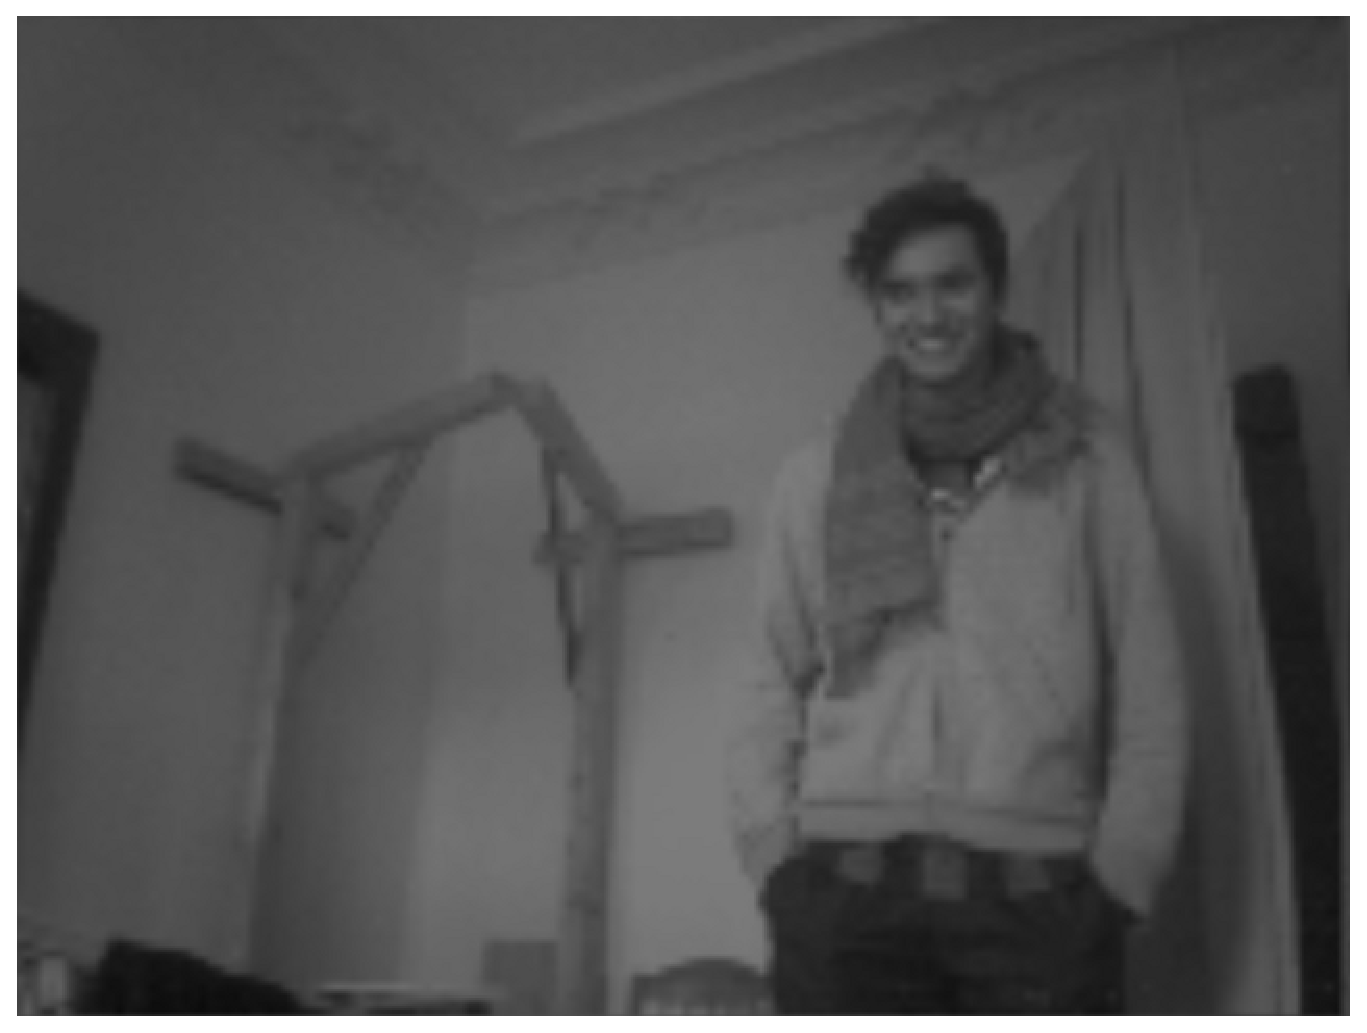
\includegraphics[width=0.3\textwidth]{img/sample-raw}}
\subfigure[2D Coder]{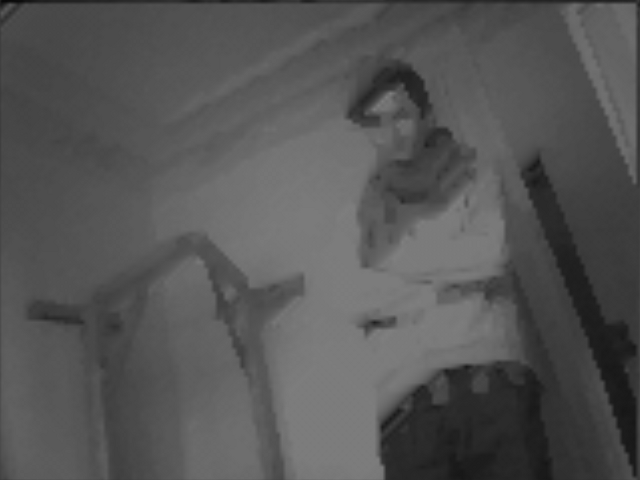
\includegraphics[width=0.3\textwidth]{img/sample-cmpr}}
\subfigure[3D Coder]{
\includegraphics[width=0.3\textwidth]{img/sample-cmpr3}}
\end{center}
\caption{Codec-Ausgabe im Vergleich zum RAW-Fromat}
\label{fig:sample}
\end{figure}

\section{Komprimierung}
\begin{table}[hp]
\centering
\begin{tabular}{|l|r|}
\hline
            & bytes/frame   \\
\hline
raw         & 19200         \\
cmpr        &  5040         \\
cmpr3 (rle) & $\approx$3200 \\
\hline
\end{tabular}
\caption{Gegen\"uberstellung der Komprimierung}
\end{table}

\section{Performance}
\begin{table}[h]
\centering
\begin{tabular}{|l|l|l|l|}
\hline
      & \multicolumn{2}{|c|}{Framerate mit Test-Video}     & \multicolumn{1}{|c|}{Rate und Frequenz mit Camera}      \\
      & mit En- und Decodierung & Encodierung und Netzwerk & Encodierung und Netzwerk \\
\hline
raw   & 133 &  52 & 10 (FREQ\_DIV = 6) \\
cmpr  &  48 &  54 & 5 (FREQ\_DIV = 12) \\
cmpr3 &  26 &  27 & 2 (FREQ\_DIV = 28) \\
\hline
\end{tabular}

\caption{Performance der Codecs, alle Angaben in Hz}
\end{table}

Leider kann die Performance nicht gut unter echten Bedingungen gemessen werden, 
da sowohl Cameramodul wie auch das Netzwerk die Datenrate begrenzen.
So zeigt nur die En- und Decodierung eines Testvideos auf dem Chip selbst zuverlässig an, wie sich die verschiedenen Kodierungen verhalten.
\\Sobald die Daten über Netzwerk übertragen werden, stellt dies zumindest bei
2D Komprimierung noch die Begrenzung da.
\\Der Test auf dem Kamerabild ist nicht aussagekräftig, 
da das Kameramodul durch die zusätzliche Last nicht schnell genug zuverlässige Bilder liefern kann. Deshalb musste die Kamerafrequenz verändert werden, was hier zur eigentlichen Begrenzung der Framerate führt.



